
\section{Fake data fit Results}

\label{app:fake_data_fit_results}

Six fake Super-K datasets at \FakePot POT were kindly made by Roger Wendell. The true input parameters 
were not revealed to the analysers until after they had been fitted by all the the groups performing a 
$\bar{\nu}_{\mu}$-disappearance analysis. The true input parameters and VALOR best-fit values for 
$\sin^{2}\overline{\theta}_{23}$ and $|\overline{\Delta m}^{2}_{32}|$ for each of these datasets are shown 
in table~\ref{tab:fake_datasets_AtoF}. The $\Delta \chi^{2}$ surfaces and confidence regions in the 
$\sin^{2}\overline{\theta}_{23}$-$|\overline{\Delta m}^{2}_{32}|$ parameter space from the fits of these datasets 
are shown in figures~\ref{fig:results_fakedata_A_chisq:normal}-\ref{fig:results_fakedata_F_contour}.

For these contours, the oscillation parameters were fixed at their values from table~\ref{tab:osc_params_fixed_values_non_reactor}.
These plots used the results of the BANFF fit to nominal MC, and version 2 of the SK Detector Errors (v3 was used for the data fit).

{
\renewcommand{\arraystretch}{1.5}
\begin{table}
\centering
\begin{tabular}{| c || c | c | c | c || c | c | c |}
\hline
 Fake      &  \multicolumn{4}{c||}{True input values} & \multicolumn{3}{c|}{VALOR best-fit values}   \\
\cline{2-8}
 dataset   &  $\sin^{2}\theta_{23}$  &  $|\Delta m^2_{32}|$ (eV$^{2}$/c$^{4}$)  & $\sin^{2}\theta_{13}$  & $\delta_{CP}$  & $\sin^{2}\overline{\theta}_{23}$  & $|\overline{\Delta m}^{2}_{32}|$ (eV$^{2}$/c$^{4}$) & Hierarchy  \\
\hline
   A       &  0.42       &  2.5$\times$10$^{-3}$   &  0.0238   &  4.712  &  0.675  &  2.774$\times$10$^{-3}$  & Inverted \\
   B       &  0.56       &  3.0$\times$10$^{-3}$   &  0.012    &  0.0    &  0.640  &  2.873$\times$10$^{-3}$  & Normal   \\
   C       &  0.52       &  2.1$\times$10$^{-3}$   &  0.0414   &  3.0    &  0.360  &  2.081$\times$10$^{-3}$  & Normal   \\
   D       &  0.63       &  -4.0$\times$10$^{-3}$  &  0.0314   &  6.01   &  0.400  &  4.160$\times$10$^{-3}$  & Inverted \\
   E       &  0.512      &  2.5$\times$10$^{-3}$   &  0.0238   &  4.712  &  0.825  &  2.576$\times$10$^{-3}$  & Normal   \\
   F       &  0.47       &  1.8$\times$10$^{-3}$   &  0.001    &  0.0    &  0.525  &  2.081$\times$10$^{-3}$  & Inverted \\
\hline
\end{tabular}
\caption{
  True input and VALOR best-fit values of oscillation parameters for Super-K fake datasets A-F.
  None of this information was known by analyzers pre-fit.
  All fake data used $\Delta m^2_{21} = 7.6 \times 10^{-5} \mathrm{eV^2}$ and $\sin^2\theta_{12}$.
}
\label{tab:fake_datasets_AtoF}
\end{table}
}

% fakedata A
%...........................................................
% 
% \Delta\chisquare surfaces 
%
\begin{figure*}[htb]
  \begin{minipage}[t]{0.96\linewidth}
    \center
    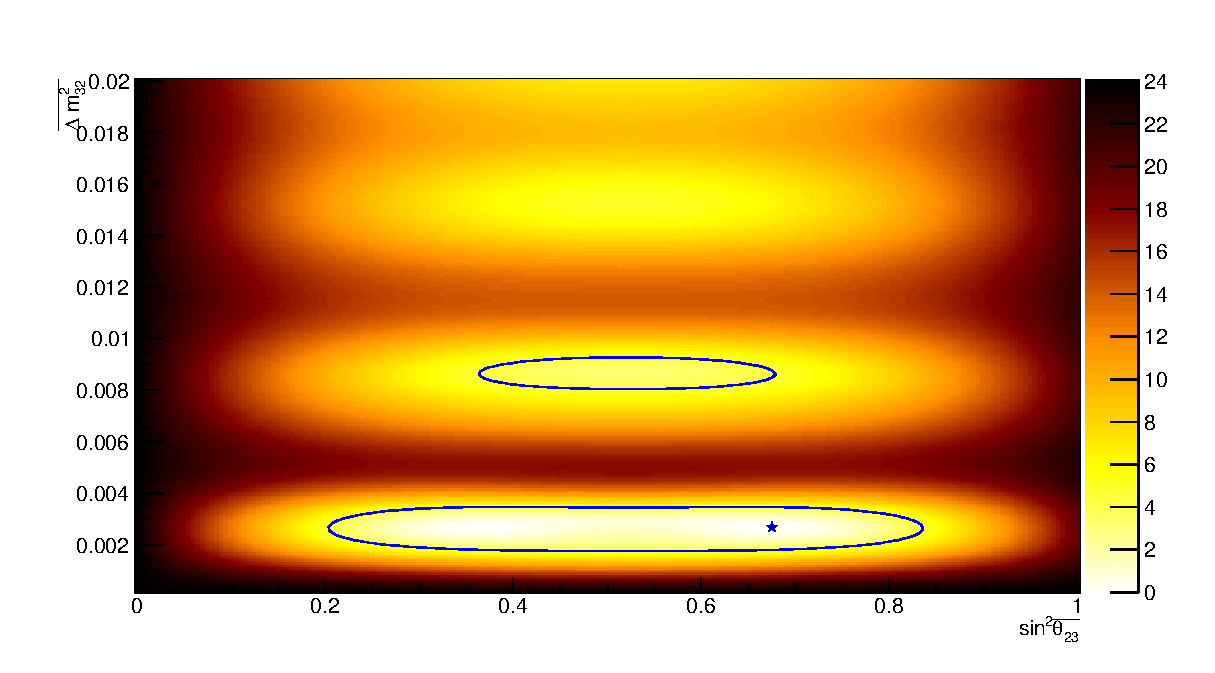
\includegraphics[width=36pc]{./images/fakedata_fit/fakedata_A_prof_nh.eps}
    \caption {
      $\Delta\chi^2$ surface from the fit of the \FakePot POT fake dataset A.
      The normal mass hierarchy is assumed.
    }
    \label{fig:results_fakedata_A_chisq:normal}
  \end{minipage}
  \vfill
  \begin{minipage}[t]{0.96\linewidth}
    \center
    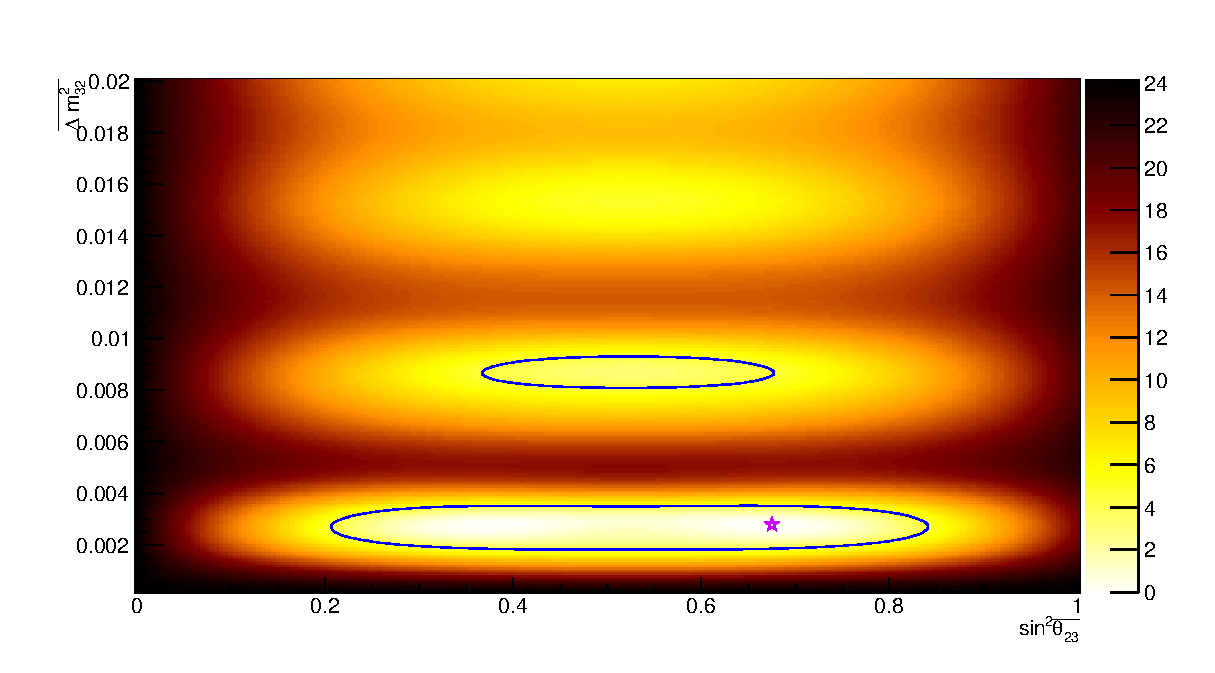
\includegraphics[width=36pc]{./images/fakedata_fit/fakedata_A_prof_ih.eps}
    \caption {
      $\Delta\chi^2$ surface from the fit of the \FakePot POT fake dataset A.
      The inverted mass hierarchy is assumed.
    }
    \label{fig:results_fakedata_A_chisq:inverted}
  \end{minipage}
\end{figure*}

\clearpage

%...........................................................
%
% Const-dchi^2 contours 
%

\clearpage

\begin{figure*}[htb]
\center
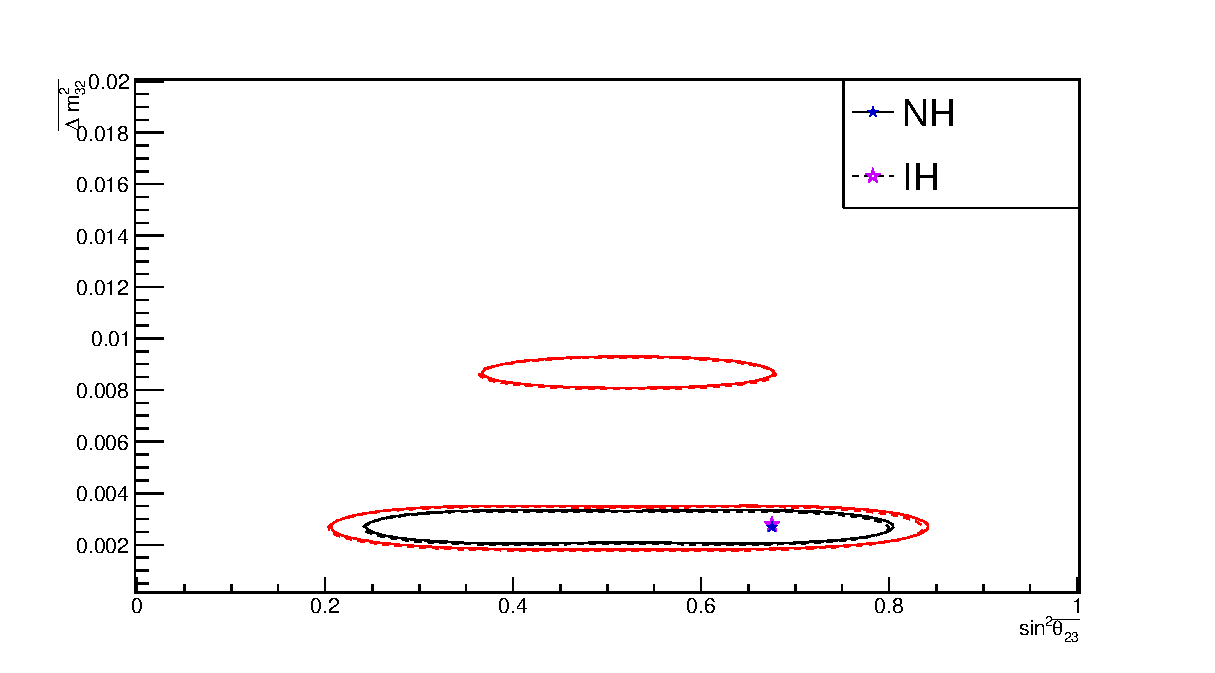
\includegraphics[width=36pc]{./images/fakedata_fit/fakedata_A_prof.eps}
\caption {
  68\% CL and 90\% CL allowed regions, 
  constructed with the constant-$\Delta\chi^{2}$ method,
  from the fit to FakePot POT fake dataset A, 
  with the effects of statistical fluctuations and postfit systematic variations being included. 
  The best-fit point for each hypothesis is shown, with the larger point representing the better of the two fits.
}
\label{fig:results_fakedata_A_contour}
\end{figure*}


% fakedata B
%...........................................................
% 
% \Delta\chisquare surfaces 
%
\begin{figure*}[htb]
  \begin{minipage}[t]{0.96\linewidth}
    \center
    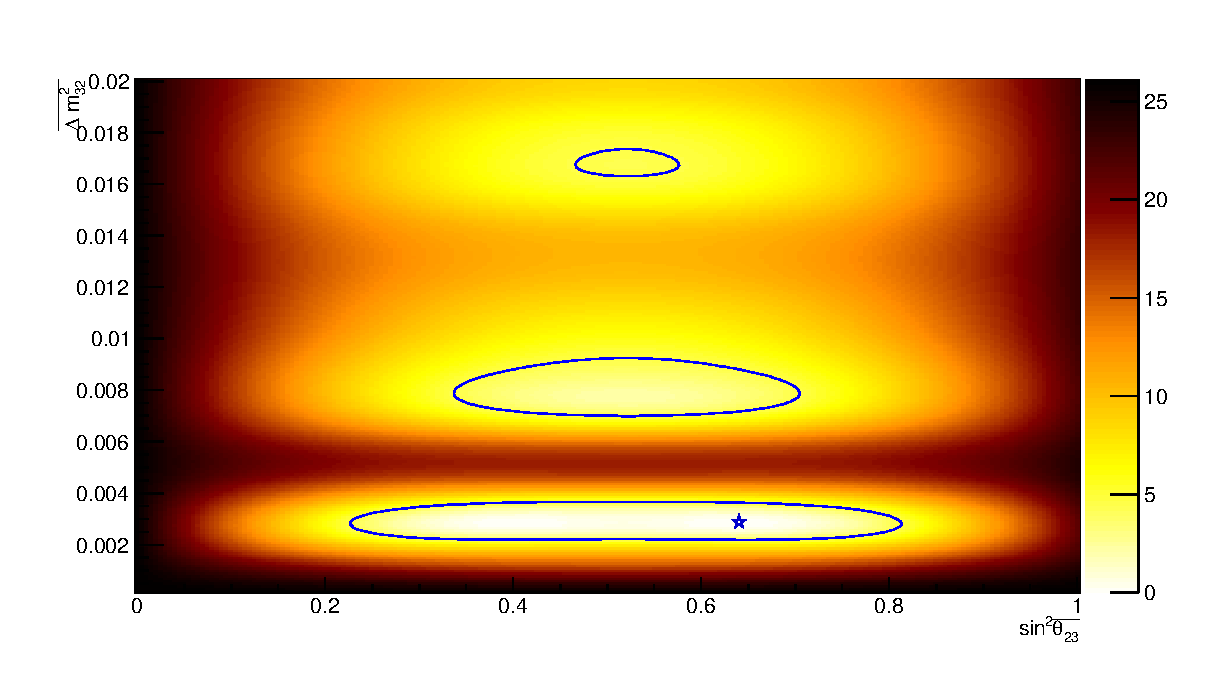
\includegraphics[width=36pc]{./images/fakedata_fit/fakedata_B_prof_nh.eps}
    \caption {
      $\Delta\chi^2$ surface from the fit of the \FakePot POT fake dataset B.
      The normal mass hierarchy is assumed.
    }
    \label{fig:results_fakedata_B_chisq:normal}
  \end{minipage}
  \vfill
  \begin{minipage}[t]{0.96\linewidth}
    \center
    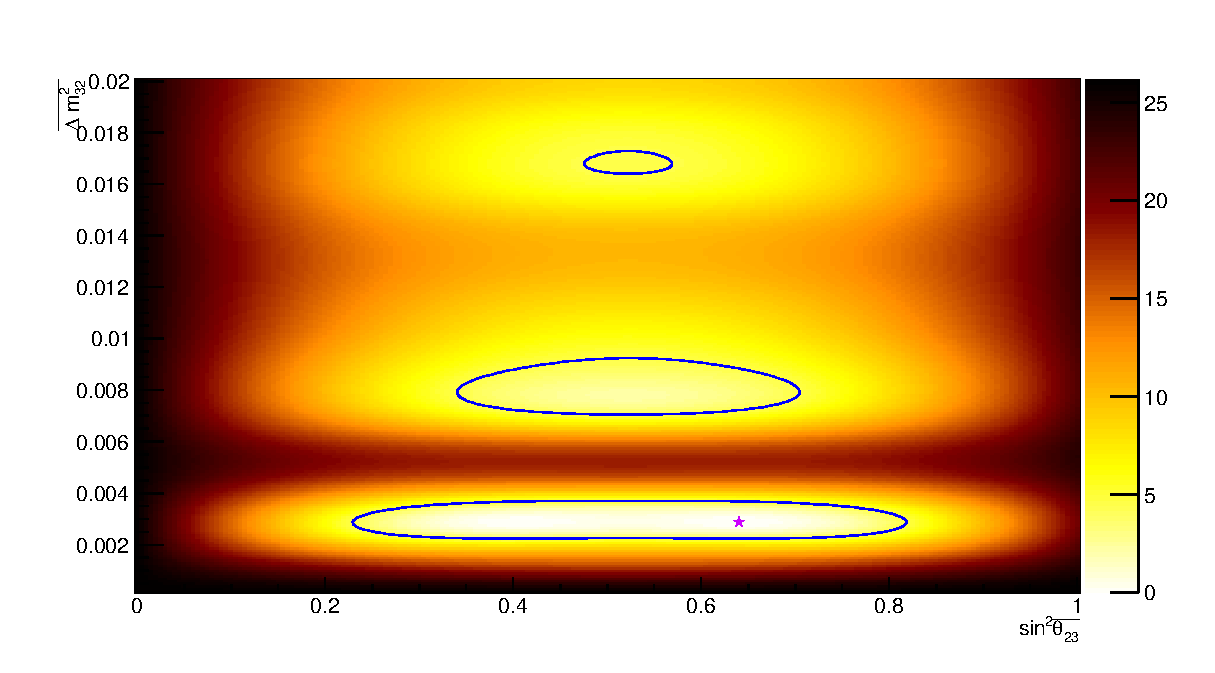
\includegraphics[width=36pc]{./images/fakedata_fit/fakedata_B_prof_ih.eps}
    \caption {
      $\Delta\chi^2$ surface from the fit of the \FakePot POT fake dataset B.
      The inverted mass hierarchy is assumed.
    }
    \label{fig:results_fakedata_B_chisq:inverted}
  \end{minipage}
\end{figure*}

\clearpage

%...........................................................
%
% Const-dchi^2 contours 
%

\clearpage

\begin{figure*}[htb]
\center
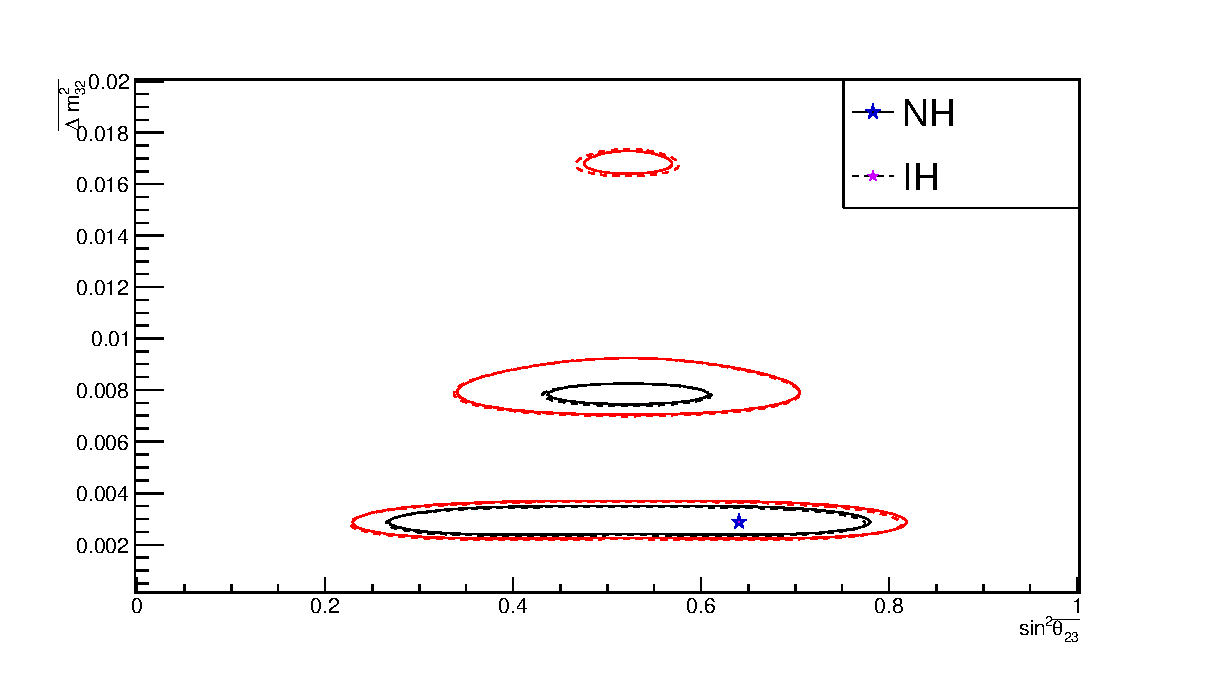
\includegraphics[width=36pc]{./images/fakedata_fit/fakedata_B_prof.eps}
\caption {
  68\% CL and 90\% CL allowed regions, 
  constructed with the constant-$\Delta\chi^{2}$ method,
  from the fit to FakePot POT fake dataset B, 
  with the effects of statistical fluctuations and postfit systematic variations being included. 
  The best-fit point for each hypothesis is shown, with the larger point representing the better of the two fits.
}
\label{fig:results_fakedata_B_contour}
\end{figure*}



% fakedata C
%...........................................................
% 
% \Delta\chisquare surfaces 
%
\begin{figure*}[htb]
  \begin{minipage}[t]{0.96\linewidth}
    \center
    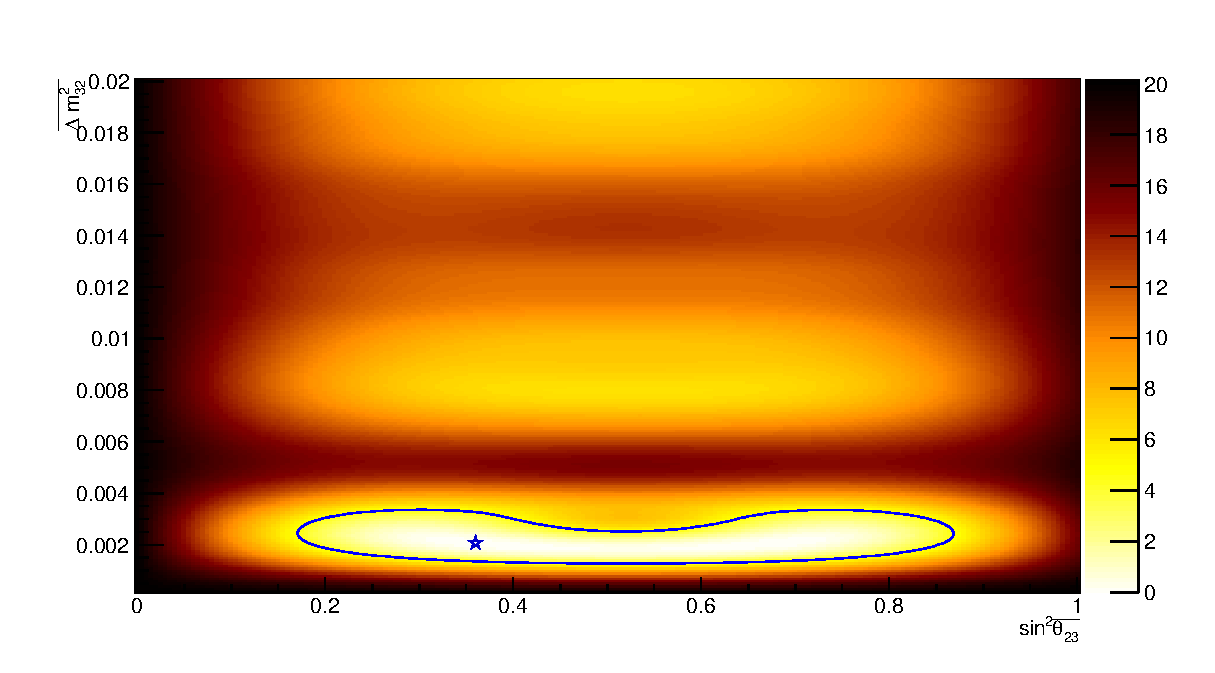
\includegraphics[width=36pc]{./images/fakedata_fit/fakedata_C_prof_nh.eps}
    \caption {
      $\Delta\chi^2$ surface from the fit of the \FakePot POT fake dataset C.
      The normal mass hierarchy is assumed.
    }
    \label{fig:results_fakedata_C_chisq:normal}
  \end{minipage}
  \vfill
  \begin{minipage}[t]{0.96\linewidth}
    \center
    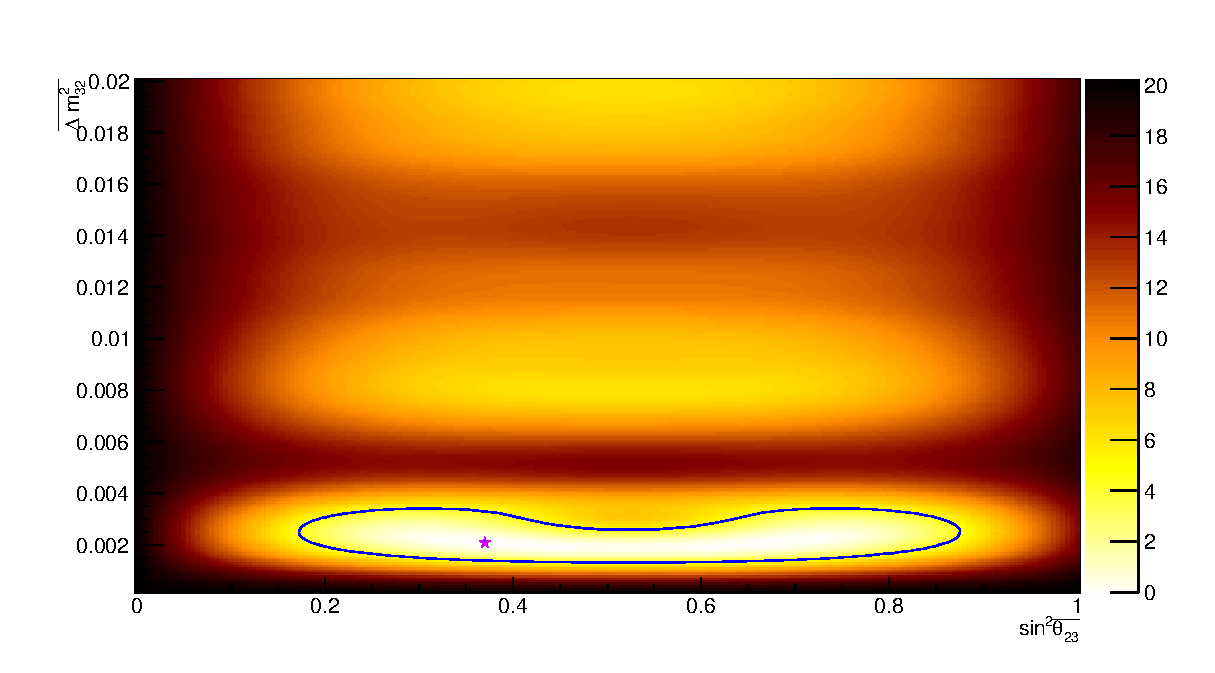
\includegraphics[width=36pc]{./images/fakedata_fit/fakedata_C_prof_ih.eps}
    \caption {
      $\Delta\chi^2$ surface from the fit of the \FakePot POT fake dataset C.
      The inverted mass hierarchy is assumed.
    }
    \label{fig:results_fakedata_C_chisq:inverted}
  \end{minipage}
\end{figure*}

\clearpage

%...........................................................
%
% Const-dchi^2 contours 
%

\clearpage

\begin{figure*}[htb]
\center
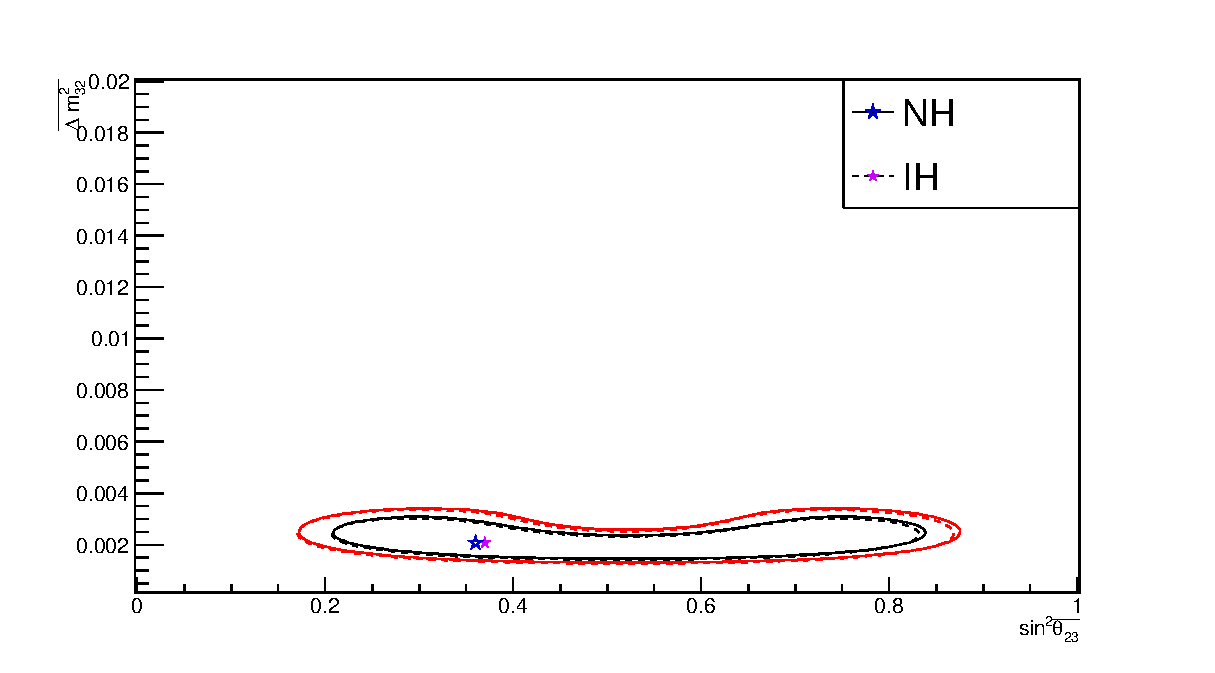
\includegraphics[width=36pc]{./images/fakedata_fit/fakedata_C_prof.eps}
\caption {
  68\% CL and 90\% CL allowed regions, 
  constructed with the constant-$\Delta\chi^{2}$ method,
  from the fit to FakePot POT fake dataset C, 
  with the effects of statistical fluctuations and postfit systematic variations being included. 
  The best-fit point for each hypothesis is shown, with the larger point representing the better of the two fits.
}
\label{fig:results_fakedata_C_contour}
\end{figure*}



% fakedata D
%...........................................................
% 
% \Delta\chisquare surfaces 
%
\begin{figure*}[htb]
  \begin{minipage}[t]{0.96\linewidth}
    \center
    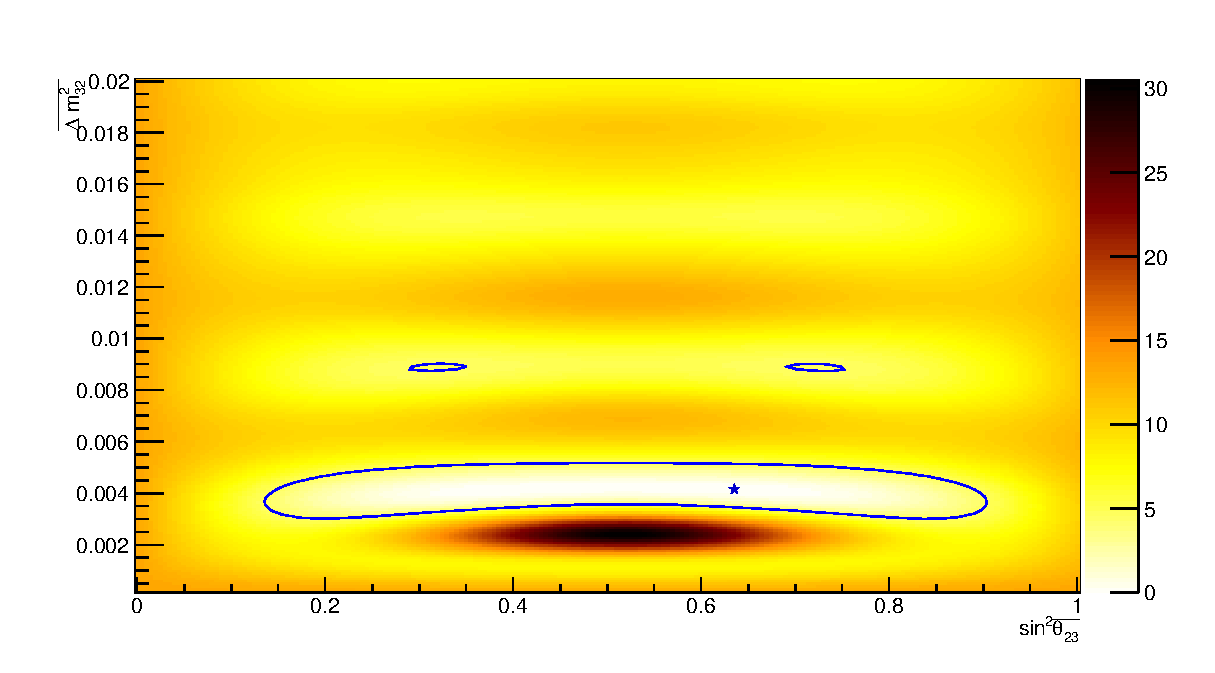
\includegraphics[width=36pc]{./images/fakedata_fit/fakedata_D_prof_nh.eps}
    \caption {
      $\Delta\chi^2$ surface from the fit of the \FakePot POT fake dataset D.
      The normal mass hierarchy is assumed.
    }
    \label{fig:results_fakedata_D_chisq:normal}
  \end{minipage}
  \vfill
  \begin{minipage}[t]{0.96\linewidth}
    \center
    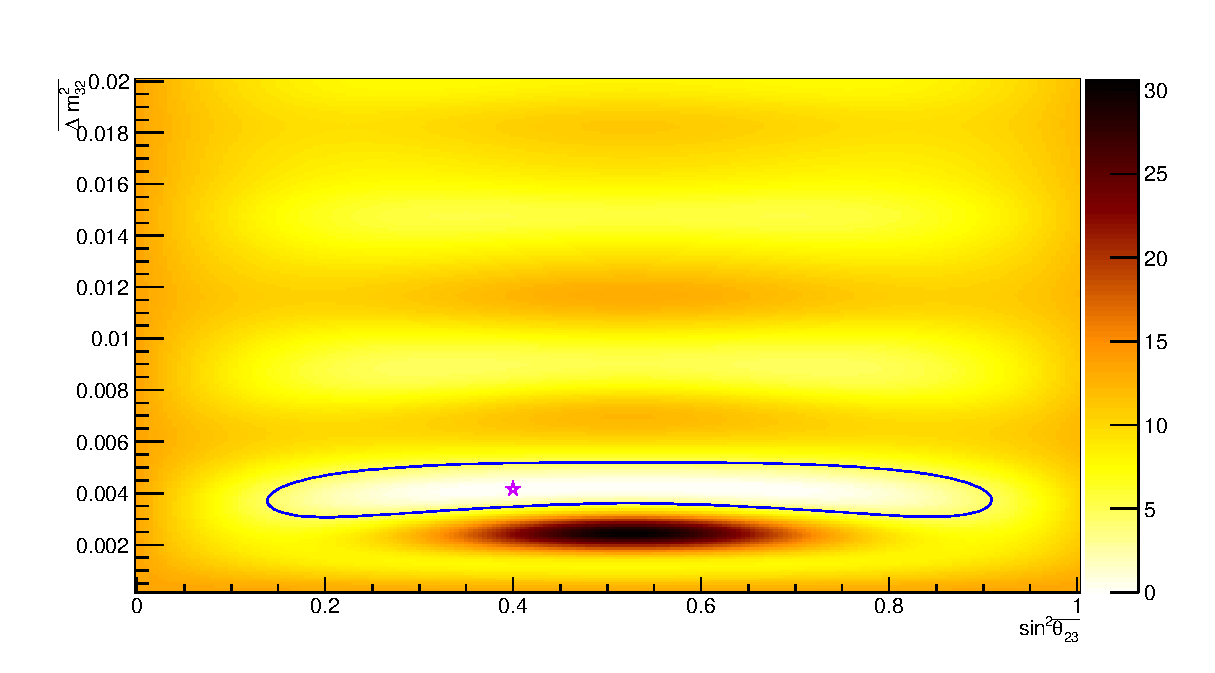
\includegraphics[width=36pc]{./images/fakedata_fit/fakedata_D_prof_ih.eps}
    \caption {
      $\Delta\chi^2$ surface from the fit of the \FakePot POT fake dataset D.
      The inverted mass hierarchy is assumed.
    }
    \label{fig:results_fakedata_D_chisq:inverted}
  \end{minipage}
\end{figure*}

\clearpage

%...........................................................
%
% Const-dchi^2 contours 
%

\clearpage

\begin{figure*}[htb]
\center
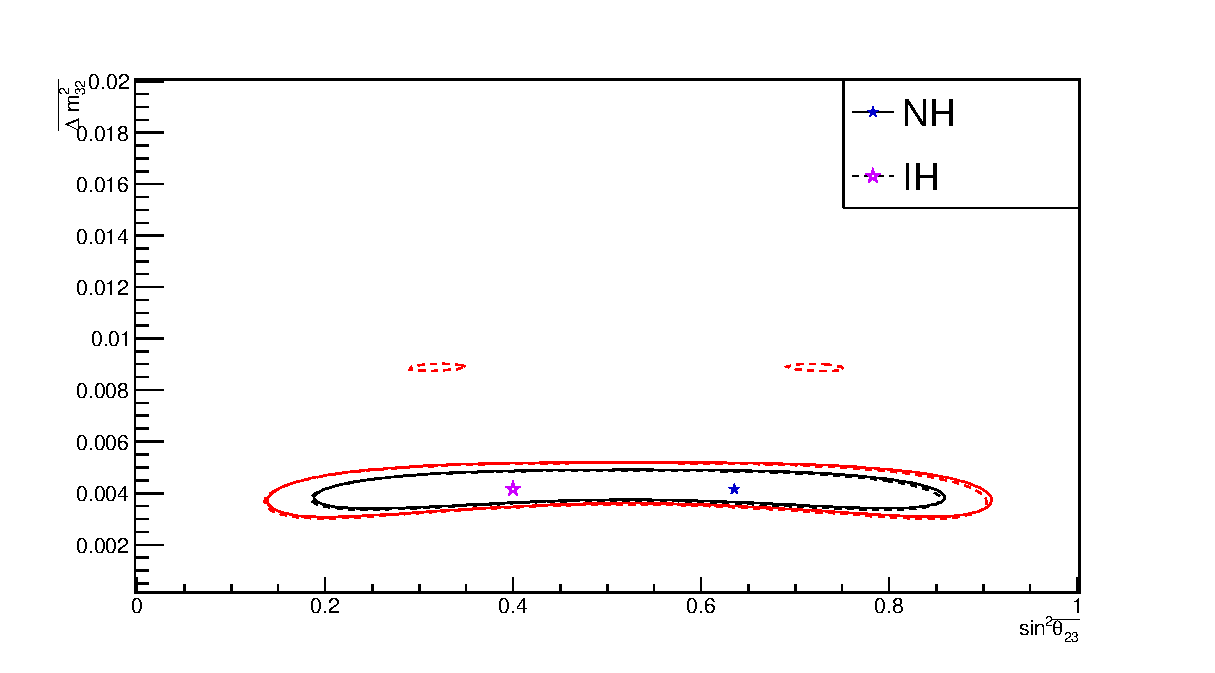
\includegraphics[width=36pc]{./images/fakedata_fit/fakedata_D_prof.eps}
\caption {
  68\% CL and 90\% CL allowed regions, 
  constructed with the constant-$\Delta\chi^{2}$ method,
  from the fit to FakePot POT fake dataset D, 
  with the effects of statistical fluctuations and postfit systematic variations being included. 
  The best-fit point for each hypothesis is shown, with the larger point representing the better of the two fits.
}
\label{fig:results_fakedata_D_contour}
\end{figure*}



% fakedata E
%...........................................................
% 
% \Delta\chisquare surfaces 
%
\begin{figure*}[htb]
  \begin{minipage}[t]{0.96\linewidth}
    \center
    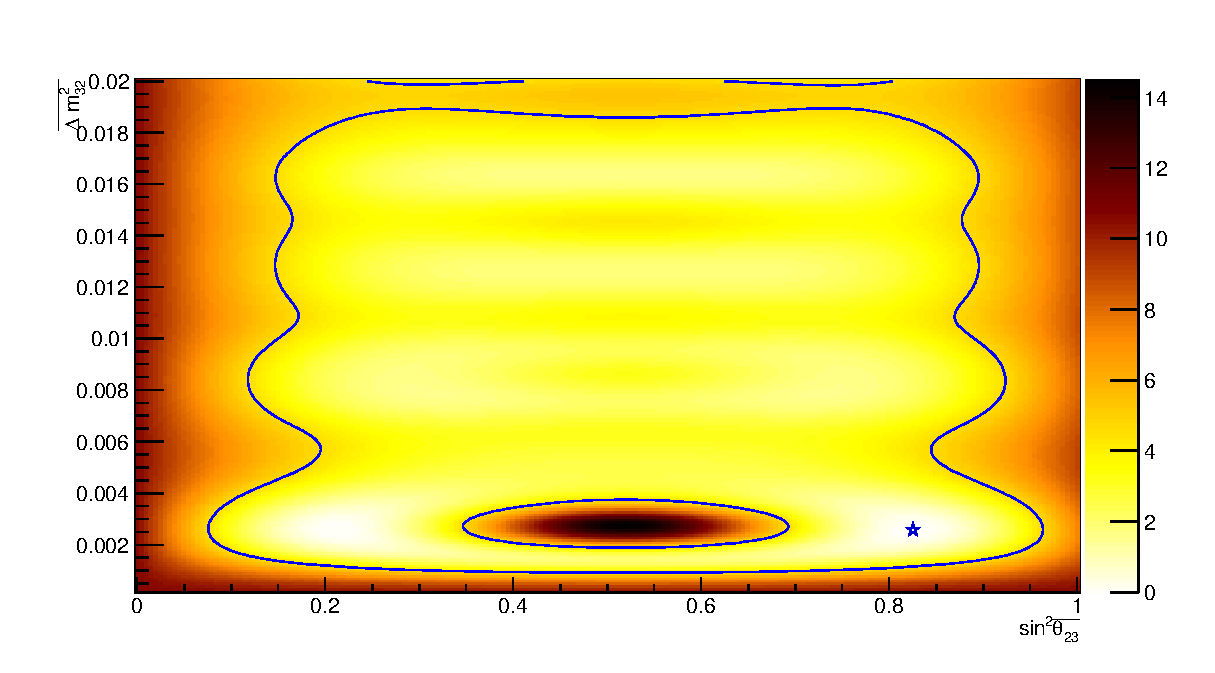
\includegraphics[width=36pc]{./images/fakedata_fit/fakedata_E_prof_nh.eps}
    \caption {
      $\Delta\chi^2$ surface from the fit of the \FakePot POT fake dataset E.
      The normal mass hierarchy is assumed.
    }
    \label{fig:results_fakedata_E_chisq:normal}
  \end{minipage}
  \vfill
  \begin{minipage}[t]{0.96\linewidth}
    \center
    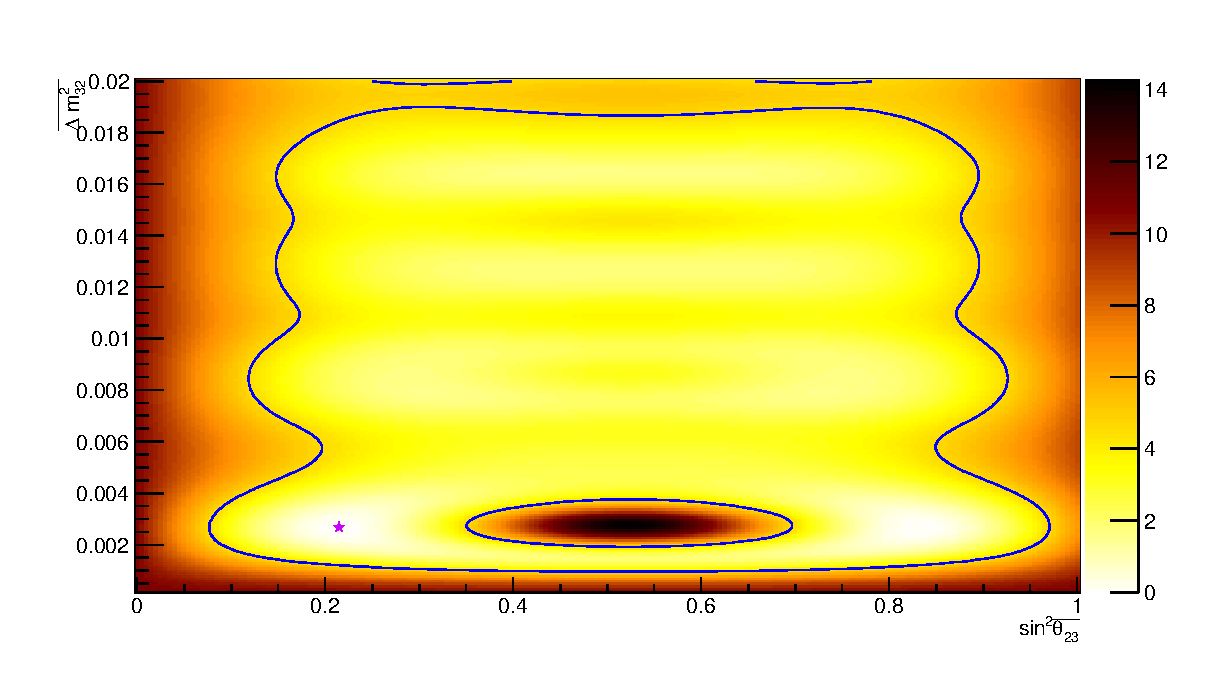
\includegraphics[width=36pc]{./images/fakedata_fit/fakedata_E_prof_ih.eps}
    \caption {
      $\Delta\chi^2$ surface from the fit of the \FakePot POT fake dataset E.
      The inverted mass hierarchy is assumed.
    }
    \label{fig:results_fakedata_E_chisq:inverted}
  \end{minipage}
\end{figure*}

\clearpage

%...........................................................
%
% Const-dchi^2 contours 
%

\clearpage

\begin{figure*}[htb]
\center
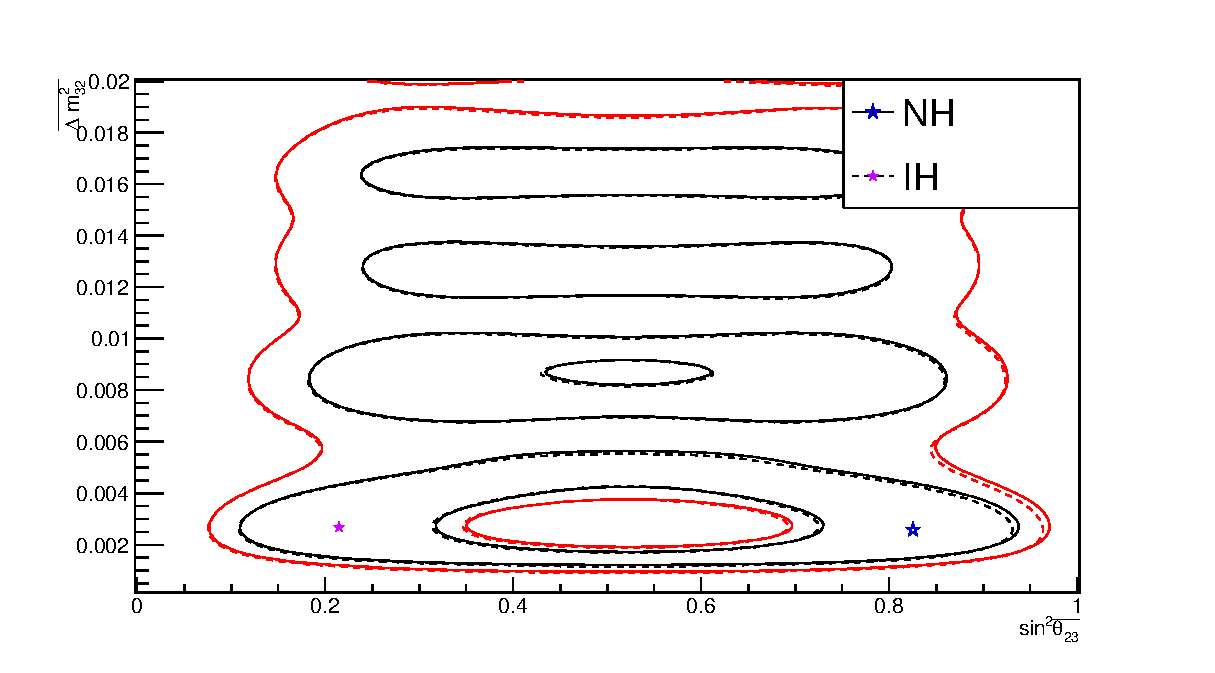
\includegraphics[width=36pc]{./images/fakedata_fit/fakedata_E_prof.eps}
\caption {
  68\% CL and 90\% CL allowed regions, 
  constructed with the constant-$\Delta\chi^{2}$ method,
  from the fit to FakePot POT fake dataset E, 
  with the effects of statistical fluctuations and postfit systematic variations being included. 
  The best-fit point for each hypothesis is shown, with the larger point representing the better of the two fits.
}
\label{fig:results_fakedata_E_contour}
\end{figure*}



% fakedata F
%...........................................................
% 
% \Delta\chisquare surfaces 
%
\begin{figure*}[htb]
  \begin{minipage}[t]{0.96\linewidth}
    \center
    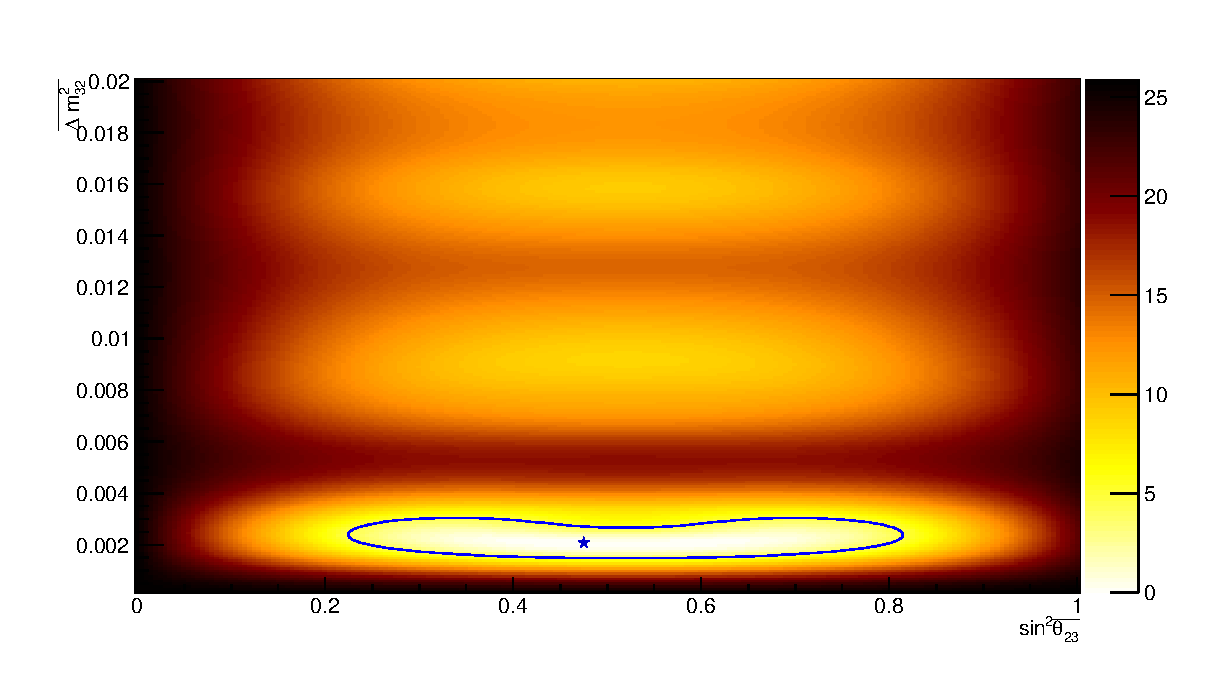
\includegraphics[width=36pc]{./images/fakedata_fit/fakedata_F_prof_nh.eps}
    \caption {
      $\Delta\chi^2$ surface from the fit of the \FakePot POT fake dataset F.
      The normal mass hierarchy is assumed.
    }
    \label{fig:results_fakedata_F_chisq:normal}
  \end{minipage}
  \vfill
  \begin{minipage}[t]{0.96\linewidth}
    \center
    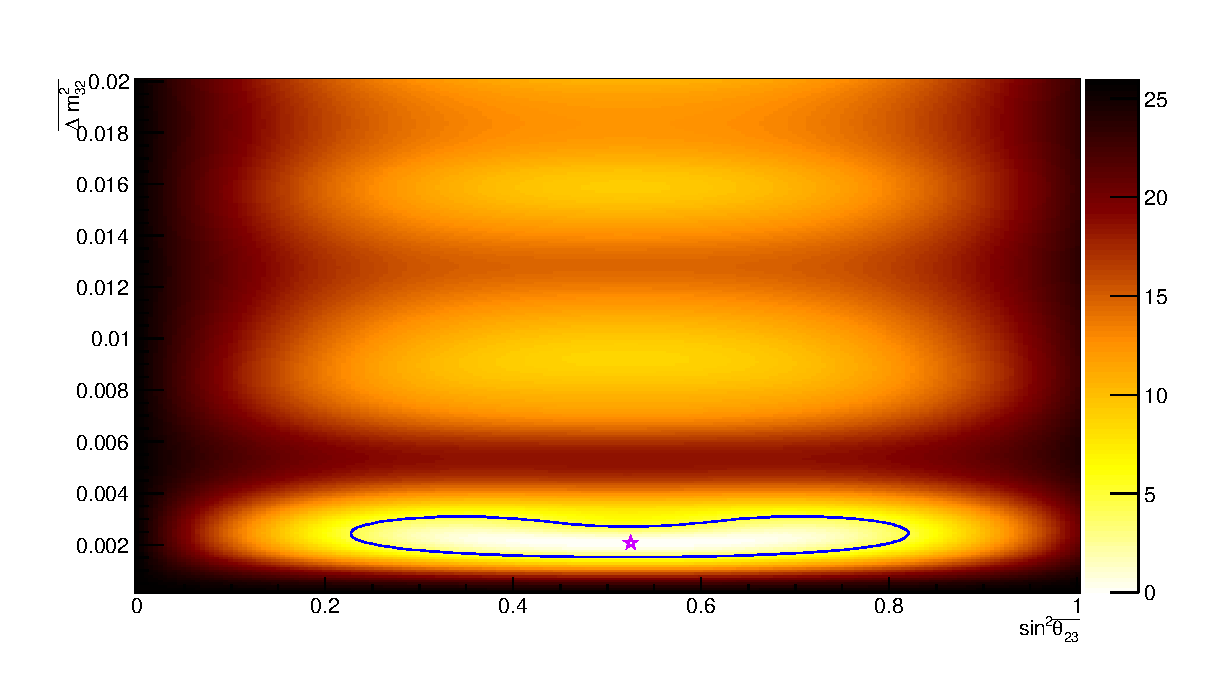
\includegraphics[width=36pc]{./images/fakedata_fit/fakedata_F_prof_ih.eps}
    \caption {
      $\Delta\chi^2$ surface from the fit of the \FakePot POT fake dataset F.
      The inverted mass hierarchy is assumed.
    }
    \label{fig:results_fakedata_F_chisq:inverted}
  \end{minipage}
\end{figure*}

\clearpage

%...........................................................
%
% Const-dchi^2 contours 
%

\clearpage

\begin{figure*}[htb]
\center
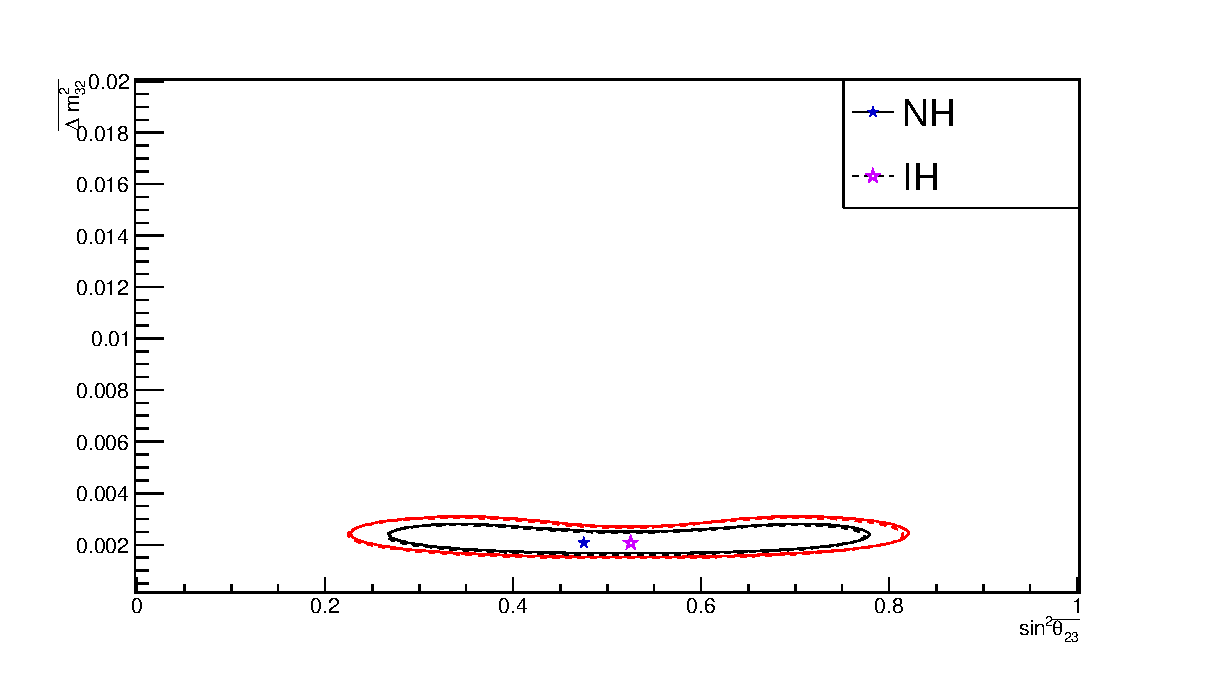
\includegraphics[width=36pc]{./images/fakedata_fit/fakedata_F_prof.eps}
\caption {
  68\% CL and 90\% CL allowed regions, 
  constructed with the constant-$\Delta\chi^{2}$ method,
  from the fit to FakePot POT fake dataset F, 
  with the effects of statistical fluctuations and postfit systematic variations being included. 
  The best-fit point for each hypothesis is shown, with the larger point representing the better of the two fits.
}
\label{fig:results_fakedata_F_contour}
\end{figure*}

